% This file was converted to LaTeX by Writer2LaTeX ver. 1.6.1
% see http://writer2latex.sourceforge.net for more info
\documentclass[a4paper]{article}
\usepackage[latin1]{inputenc}
\usepackage{amsmath}
\usepackage{amssymb,amsfonts,textcomp}
\usepackage[T1]{fontenc}
\usepackage[english]{babel}
\usepackage{color}
\usepackage{array}
\usepackage{supertabular}
\usepackage{hhline}
\usepackage{hyperref}
\hypersetup{pdftex, colorlinks=true, linkcolor=blue, citecolor=blue, filecolor=blue, urlcolor=blue, pdftitle=, pdfauthor=Jordan Taylor, pdfsubject=, pdfkeywords=}
\usepackage[pdftex]{graphicx}
\providecommand\textsubscript[1]{\ensuremath{{}_{\text{#1}}}}
% Outline numbering
\setcounter{secnumdepth}{0}
\makeatletter
\newcommand\arraybslash{\let\\\@arraycr}
\makeatother
% Page layout (geometry)
\setlength\voffset{-1in}
\setlength\hoffset{-1in}
\setlength\topmargin{1.251cm}
\setlength\oddsidemargin{2.501cm}
\setlength\textheight{22.396004cm}
\setlength\textwidth{15.999001cm}
\setlength\footskip{2.401cm}
\setlength\headheight{1.251cm}
\setlength\headsep{1.15cm}
% Footnote rule
\setlength{\skip\footins}{0.119cm}
\renewcommand\footnoterule{\vspace*{-0.018cm}\setlength\leftskip{0pt}\setlength\rightskip{0pt plus 1fil}\noindent\textcolor{black}{\rule{0.25\columnwidth}{0.018cm}}\vspace*{0.101cm}}
% Pages styles
\makeatletter
\newcommand\ps@Standard{
  \renewcommand\@oddhead{[Warning: Draw object ignored]}
  \renewcommand\@evenhead{\@oddhead}
  \renewcommand\@oddfoot{\textstylepagenumber{\thepage{}}}
  \renewcommand\@evenfoot{\@oddfoot}
  \renewcommand\thepage{\arabic{page}}
}
\makeatother
\pagestyle{Standard}
\setlength\tabcolsep{1mm}
\renewcommand\arraystretch{1.3}
% List styles
\newcounter{saveenum}
\newcommand\liststyleWWNumxiii{%
\renewcommand\labelitemi{[F0B7?]}
\renewcommand\labelitemii{o}
\renewcommand\labelitemiii{[F0A7?]}
\renewcommand\labelitemiv{[F0B7?]}
}
\newcommand\liststyleWWNumxxi{%
\renewcommand\labelitemi{[F0B7?]}
\renewcommand\labelitemii{o}
\renewcommand\labelitemiii{[F0A7?]}
\renewcommand\labelitemiv{[F0B7?]}
}
\newcommand\liststyleWWNumxxiii{%
\renewcommand\theenumi{\arabic{enumi}}
\renewcommand\theenumii{\arabic{enumi}.\arabic{enumii}}
\renewcommand\theenumiii{\arabic{enumi}.\arabic{enumii}.\arabic{enumiii}}
\renewcommand\theenumiv{\arabic{enumi}.\arabic{enumii}.\arabic{enumiii}.\arabic{enumiv}}
\renewcommand\labelenumi{\theenumi}
\renewcommand\labelenumii{\theenumii}
\renewcommand\labelenumiii{\theenumiii}
\renewcommand\labelenumiv{\theenumiv}
}
\newcommand\liststyleWWNumxxvii{%
\renewcommand\labelitemi{[F0B7?]}
\renewcommand\labelitemii{o}
\renewcommand\labelitemiii{[F0A7?]}
\renewcommand\labelitemiv{[F0B7?]}
}
\newcommand\liststyleWWNumv{%
\renewcommand\labelitemi{[F0B7?]}
\renewcommand\labelitemii{o}
\renewcommand\labelitemiii{[F0A7?]}
\renewcommand\labelitemiv{[F0B7?]}
}
\newcommand\liststyleWWNumxviii{%
\renewcommand\theenumi{\arabic{enumi}}
\renewcommand\labelenumi{\theenumi.}
\renewcommand\labelitemi{o}
\renewcommand\labelitemii{[F0A7?]}
\renewcommand\labelitemiii{[F0B7?]}
}
\newcommand\liststyleWWNumxx{%
\renewcommand\theenumi{\arabic{enumi}}
\renewcommand\labelenumi{\theenumi.}
\renewcommand\labelitemi{o}
\renewcommand\labelitemii{[F0A7?]}
\renewcommand\labelitemiii{[F0B7?]}
}
\newcommand\liststyleWWNumxix{%
\renewcommand\labelitemi{[F0B7?]}
\renewcommand\labelitemii{o}
\renewcommand\labelitemiii{[F0A7?]}
\renewcommand\labelitemiv{[F0B7?]}
}
% Non-floating captions
\makeatletter
\newcommand\captionof[1]{\def\@captype{#1}\caption}
\makeatother
\newcounter{Algorithm}
\renewcommand\theAlgorithm{\arabic{Algorithm}}
\newcounter{Listing}
\renewcommand\theListing{\arabic{Listing}}
\title{}
\author{Jordan Taylor}
\date{2023-03-25}
\begin{document}
\clearpage\setcounter{page}{1}\pagestyle{Standard}

\bigskip


\bigskip



\begin{figure}
\centering

\includegraphics[width=4.625cm,height=1.342cm]{Gimbalscope20Dissertation20PreTex-img001.png}
\end{figure}

\bigskip


\bigskip


\bigskip


\bigskip

{\centering
\textcolor{black}{DEPARTMENT OF COMPUTER SCIENCE}
\par}


\bigskip


\bigskip


\bigskip

{\centering
\textcolor{black}{GIMBALSCOPE: SPACECRAFT ATTITUDE CONTROL FOR HAPTIC FEEDBACK}
\par}

{\centering
\textcolor{black}{A Dual Parallel Gimbal Controlled Moment Gyroscope for Ungrounded Directional Force Feedback}
\par}


\bigskip


\bigskip


\bigskip

{\centering
\textcolor{black}{Jordan Taylor}
\par}


\bigskip


\bigskip


\bigskip


\bigskip

{\centering [Warning: Draw object ignored]\par}

\bigskip

{\centering
\textcolor{black}{A dissertation submitted to the University of Bristol in accordance with the requirements of the
degree}
\par}

{\centering
\textcolor{black}{of Master of Engineering in the Faculty of Engineering.}
\par}

{\centering [Warning: Draw object ignored]\par}

\bigskip


\bigskip

{\centering
\textcolor{black}{Wednesday, 16 March 2022}
\par}


\bigskip

\clearpage
\bigskip

Abstract


\bigskip


\bigskip

\textbf{A compulsory section, of at most 300 words}


\bigskip


\bigskip

This section should precis the project context, aims and objectives, and main contributions (e.g., deliverables) and
achievements; the same section may be called an abstract elsewhere. The goal is to ensure the reader is clear about
what the topic is, what you have done within this topic, and what your view of the outcome is.


\bigskip

The former aspects should be guided by your specification: essentially this section is a (very) short version of what is
typically the first chapter. Note that for research-type projects, this must include a clear research hypothesis. This
will obviously differ significantly for each project, but an example might be as follows:


\bigskip

My research hypothesis is that a suitable genetic algorithm will yield more accurate results

(when applied to the standard ACME data set) than the algorithm proposed by Jones and

Smith, while also executing in less time.


\bigskip

The latter aspects should (ideally) be presented as a concise, factual bullet point list. Again, the points will differ
for each project, but an might be as follows:


\bigskip

\liststyleWWNumxiii
\begin{itemize}
\item I spent 120 hours collecting material on and learning about the Java garbage-collection sub-system.
\item I wrote a total of 5000 lines of source code, comprising a Linux device driver for a robot (in C) and a GUI (in
Java) that is used to control it.
\item I designed a new algorithm for computing the non-linear mapping from A-space to B-space using a genetic algorithm,
see page 17.
\item I implemented a version of the algorithm proposed by Jones and Smith in [6], see page 12, corrected a mistake in
it, and compared the results with several alternatives.
\end{itemize}
\clearpage\section{Dedication and Acknowledgements}
\hypertarget{Toc98342026}{}
\bigskip

\textbf{A compulsory section}


\bigskip

I would like to express my appreciation for the Teaching Technologist Team at the University of Bristol, with particular
note for the Hackspace. Although not having a direct influence in this Dissertation, I would not be equipped with the
practical engineering skills I have today without the opportunity to learn-through-doing afforded by the team.


\bigskip

A massive thank you to my Mother, Father, and The Computer Science Year 4 Pastoral Tutor Chris Priest for supporting and
enabling a part-time schedule of study as I deal with post-covid health issues.


\bigskip

Finally, an additional thanks to BIG (Bristol Interaction Group) for facilitating my work and being a bunch of wonderful
people.


\bigskip


\bigskip

\clearpage
Declaration


\bigskip


\bigskip

I declare that the work in this dissertation was carried out in accordance with the requirements of the University's
Regulations and Code of Practice for Taught Programmes and that it has not been submitted for any other academic award.
Except where indicated by specific reference in the text, this work is my own work. Work done in collaboration with, or
with the assistance of others, is indicated as such. I have identified all material in this dissertation which is not
my own work through appropriate referencing and acknowledgement. Where I have quoted or otherwise incorporated material
which is the work of others, I have included the source in the references. Any views expressed in the dissertation,
other than referenced material, are those of the author.


\bigskip


\bigskip


\bigskip

Jordan Taylor, Wednesday, 1\textsuperscript{st} May 2023


\bigskip

\clearpage\section{Contents}

\bigskip


\bigskip

\setcounter{tocdepth}{3}
\renewcommand\contentsname{}
\tableofcontents

\bigskip


\bigskip


\bigskip


\bigskip


\bigskip

\clearpage\section{List of Figures}
\hypertarget{Toc98342027}{}
\bigskip

\listoffigures

\bigskip


\bigskip


\bigskip

\clearpage\section{}
\section{List of Tables}
\hypertarget{Toc98342028}{}
\bigskip


\bigskip

\listoffigures

\bigskip


\bigskip


\bigskip

\clearpage\section{}
Ethics Statement


\bigskip


\bigskip

This project did not require ethical review, as determined by my supervisor, Anne Roudaut.\textcolor{black}{ }

\clearpage\section{Supporting Technologies}
\hypertarget{Toc98342030}{}
\bigskip

\liststyleWWNumxxi
\begin{itemize}
\item \textcolor{black}{I used a pair of standard 1806 2300Kv brushless motors as the core of the gyroscope rotors.}
\item \textcolor{black}{I used a pair of 12V Micro Metal Geared Motors with Quadrature Encoders at 210:1 reduction for
actuating the outer gimbals.}
\item \textcolor{black}{I used a Bluebird BMS-620MG Metal Gear Analogue Servo for actuating the central gimbal.}
\item \textcolor{black}{I used a pair of Adafruit RFM69HCW 900MHz Radio Transceivers for wireless communication between
the Gimbalscope and PC in conjunction with the official RH\_RF69 radio driver library.}
\item \textcolor{black}{I used a pair of Arduino Mega 2560 Rev3s to provide a platform for Gimbalscope control and PC
communication dongle.}
\item \textcolor{black}{I used an Arduino Micro in the role of The Gimbalscope's dedicated radio transceiver operator.}
\item \textcolor{black}{I used an Adafruit L3GD20H Triple-Axis Gyro Breakout Board in conjunction with the Unified
L3GD20 driver library for Gimbalscope orientation tracking.}
\item \textcolor{black}{I used a standard MPU-6050 breakout board to provide a platform for vibration and gyroscopic
force measurements.}
\item \textcolor{black}{I used Microsoft 3D builder and Autodesk Fusion 360 to design the 3D printed parts used in the
creation of The Gimbalscope.}
\item \textcolor{black}{I used an Ultimaker 2 Extended + 3D printer to print the 3D printed parts used in The
Gimbalscope.}
\item \textcolor{black}{I used the Unity Real-Time Development Platform in conjunction with the Ardity Arduino Serial
Package to create bespoke Gimbalscope control software.}
\item \textcolor{black}{I used NumPy and matplotlib Python libraries to compute and plot results from user trials, as
well as vibration and gyroscopic force data.}
\end{itemize}

\bigskip


\bigskip


\bigskip

\clearpage\section{Notions and Acronyms}
\hypertarget{Toc98342031}{}
\bigskip

\textbf{\textcolor{black}{An optional section}}


\bigskip

\begin{flushleft}
\tablefirsthead{}
\tablehead{}
\tabletail{}
\tablelasttail{}
\begin{supertabular}{m{1.52cm}m{0.32200003cm}m{13.557cm}}
\raggedleft{\selectlanguage{english}\bfseries \textcolor{black}{CMG}} &
{\selectlanguage{english}\bfseries \textcolor{black}{:}} &
{\selectlanguage{english} \textcolor{black}{Controlled Moment Gyroscope}}\\
\raggedleft{\selectlanguage{english}\bfseries \textcolor{black}{DCMG}} &
{\selectlanguage{english} \textcolor{black}{:}} &
{\selectlanguage{english} \textcolor{black}{Dual Controlled Moment Gyroscope}}\\
\raggedleft{\selectlanguage{english}\bfseries \textcolor{black}{LED \ }} &
{\selectlanguage{english} \textcolor{black}{:}} &
{\selectlanguage{english} \textcolor{black}{Light Emitting Diode}}\\
\raggedleft{\selectlanguage{english}\bfseries \textcolor{black}{RPM \ }} &
{\selectlanguage{english} \textcolor{black}{:}} &
{\selectlanguage{english} \textcolor{black}{Revolutions-Per-Minute}}\\
\raggedleft{\selectlanguage{english}\bfseries \textcolor{black}{Kv \ }} &
{\selectlanguage{english} \textcolor{black}{:}} &
{\selectlanguage{english} \textcolor{black}{Estimation of RPM-per-Volt of a brushless motor in a no-load condition.}}\\
\raggedleft{\selectlanguage{english}\bfseries \textcolor{black}{ESC}} &
{\selectlanguage{english} \textcolor{black}{:}} &
{\selectlanguage{english} \textcolor{black}{Electronic Speed Controller. Governs speed of a motor.}}\\
\raggedleft{\selectlanguage{english}\bfseries \textcolor{black}{BEC}} &
{\selectlanguage{english} \textcolor{black}{:}} &
{\selectlanguage{english} \textcolor{black}{Battery Eliminator Circuit. Regulates voltage to connected circuit.}}\\
\raggedleft{\selectlanguage{english}\bfseries \textcolor{black}{PWM}} &
{\selectlanguage{english} \textcolor{black}{:}} &
{\selectlanguage{english} \textcolor{black}{Pulse Width Modulation. Digital square wave with duty cycle to imitate
analogue control signals.}}\\
\raggedleft{\selectlanguage{english}\bfseries \textcolor{black}{PLA \ }} &
{\selectlanguage{english} \textcolor{black}{:}} &
{\selectlanguage{english} \textcolor{black}{Polylactic acid, a commonly used bioplastic 3D printing filament.}}\\
\raggedleft{\selectlanguage{english}\bfseries \textcolor{black}{PID}} &
{\selectlanguage{english} \textcolor{black}{:}} &
{\selectlanguage{english} \textcolor{black}{Proportional-integral-derivative controller; a mechanical control loop
mechanism.}}\\
\raggedleft{\selectlanguage{english}\bfseries \textcolor{black}{IMU}} &
{\selectlanguage{english} \textcolor{black}{:}} &
{\selectlanguage{english} \textcolor{black}{Inertial Measurement Unit -- a combined electronic apparatus using a
combination of accelerometers and gyroscopes to report forces and angular rates.}}\\
\raggedleft{\selectlanguage{english}\bfseries
\textcolor{black}{I}\textcolor{black}{\textsuperscript{2}}\textcolor{black}{C}} &
{\selectlanguage{english} \textcolor{black}{:}} &
{\selectlanguage{english} \textcolor{black}{Inter-Integrated Circuit. A synchronous multi-master/multi-slave
communication bus. Used by Arduino boards to communicate with a number of peripheral devices.}}\\
\raggedleft{\selectlanguage{english}\bfseries \textcolor{black}{SPI}} &
{\selectlanguage{english} \textcolor{black}{:}} &
{\selectlanguage{english} \textcolor{black}{Serial Parallel Interface. Single master/multi-slave setup. Synchronous
serial communication protocol. Data transfer is timed with clock pulses.}}\\
\raggedleft{\selectlanguage{english}\bfseries \textcolor{black}{MOSI}} &
{\selectlanguage{english} \textcolor{black}{:}} &
{\selectlanguage{english} \textcolor{black}{Part of }\textbf{\textcolor{black}{SPI}}\textcolor{black}{. Master Out Slave
In. Connection from master device to slave device.}}\\
\raggedleft{\selectlanguage{english}\bfseries \textcolor{black}{MISO}} &
{\selectlanguage{english} \textcolor{black}{:}} &
{\selectlanguage{english} \textcolor{black}{Part of
}\textbf{\textcolor{black}{SPI}}\textcolor{black}{.}\textbf{\textcolor{black}{ }}\textcolor{black}{Master In Slave Out.
Connection from slave device to master device.}}\\
\raggedleft{\selectlanguage{english}\bfseries \textcolor{black}{SCLK}} &
{\selectlanguage{english} \textcolor{black}{:}} &
{\selectlanguage{english} \textcolor{black}{Part of }\textbf{\textcolor{black}{SPI}}\textcolor{black}{. Serial Clock
pulse carrier.}}\\
\raggedleft{\selectlanguage{english}\bfseries \textcolor{black}{CS}} &
{\selectlanguage{english} \textcolor{black}{:}} &
{\selectlanguage{english} \textcolor{black}{Part of }\textbf{\textcolor{black}{SPI}}\textcolor{black}{. Chip Select.
Connection from master device to slave device to inform an imminent send or request of data.}}\\
\end{supertabular}
\end{flushleft}

\bigskip


\bigskip


\bigskip


\bigskip


\bigskip


\bigskip


\bigskip


\bigskip


\bigskip


\bigskip


\bigskip


\bigskip


\bigskip


\bigskip

\section[Chapter 1:]{\textbf{Chapter 1:}}
\hypertarget{Toc98342032}{}\section[Introduction ]{\textbf{Introduction}\textbf{ }}

\bigskip


\bigskip

\textcolor{black}{A key problem with current force feedback haptic devices is balancing the three-way tradeoff between
form factor, workspace of interaction, and force fidelity. It is difficult to design a device with two of these tenets
without sacrificing the third. In the hands of a user, the quality of a device can be evaluated as a function of all
three.}

\textcolor{black}{\ \ Conventional high-fidelity haptic feedback devices tend to rely on transmitting ground-based
reaction forces to the user via a series of rigid joints and links, thus restricting their portability. Contrastingly,
ungrounded haptic feedback devices afford users with kinesthetic or tactile feedback over a wider workspace. Despite
this, many approaches to portable haptic feedback are designed to solely stimulate the skin, through means such as
vibration}\cite{CITATIONTOr07l2057}\textcolor{black}{, skin deformation}\cite{CITATIONTSm20l2057}\textcolor{black}{ ,
or shape alteration
}\cite{CITATIONAJS17l2057}\cite{CITATIONCSw03l2057}\textcolor{black}{\ }\cite{CITATIONAZe19l2057}\textcolor{black}{.
\ These devices have many benefits such as their small size, light weight. However, according to Haptipdeia
}\cite{CITATIONHas19l2057}\textcolor{black}{\ {}- the database of haptic devices -- there are very few ungrounded
handheld devices capable of directional force feedback, and even fewer capable of three-degrees-of-freedom forces.}

\textcolor{black}{\ \ A solution to this is the use of DCMGs (Dual Controlled Moment Gyroscopes). DCMGs are a form of
gyroscope that use a pair of counter-rotating flywheels to induce a torque about an arbitrary axis, and are most
commonly used in spacecraft attitude control systems }\cite{CITATIONPCu14l2057}\textcolor{black}{.}

\textcolor{black}{\ \ This dissertation presents a prototype handheld DCMG-based haptic device nicknamed
}\textit{\textcolor{black}{{}`The Gimbalscope'}}\textcolor{black}{. Truly ungrounded, remotely operated, and battery
powered, }\textit{\textcolor{black}{The Gimbalscope }}\textcolor{black}{seeks to make a novel contribution to the field
of ungrounded haptics, as well as increase the accessibility of performing such research with its low-cost,
open-standard components and open-source implementation. }\textit{\textcolor{black}{The Gimbalscope
}}\textcolor{black}{shall be evaluated}\textit{\textcolor{black}{ }}\textcolor{black}{in a variety of experiments
designed to quantify the ability of humans to perceive torque generated from an ungrounded DCMG haptic feedback
device.}


\bigskip


\bigskip

\textbf{1.1 \ \ Aims and Objectives}


\bigskip

\liststyleWWNumxxiii
\begin{enumerate}
\item Produce a working battery powered Dual Controlled Moment Gyroscope.
\end{enumerate}

\bigskip

\liststyleWWNumxxiii
\setcounter{saveenum}{\value{enumi}}
\begin{enumerate}
\setcounter{enumi}{\value{saveenum}}
\item Wirelessly control the device from a computer.
\end{enumerate}

\bigskip

\liststyleWWNumxxiii
\setcounter{saveenum}{\value{enumi}}
\begin{enumerate}
\setcounter{enumi}{\value{saveenum}}
\item Evaluate the ability for users to perceive a range of torques in three degrees-of-freedom.
\end{enumerate}

\bigskip

\liststyleWWNumxxiii
\setcounter{saveenum}{\value{enumi}}
\begin{enumerate}
\setcounter{enumi}{\value{saveenum}}
\item Evaluate the ability of users to use \textit{The Gimbalscope} in real-world target identification scenarios.
\end{enumerate}

\bigskip


\bigskip


\bigskip


\bigskip


\bigskip


\bigskip


\bigskip


\bigskip


\bigskip

\section[Chapter 2:]{\textbf{Chapter 2:}}
\hypertarget{Toc98342033}{}\section[Background]{\textbf{Background}}
\section[Related Work]{\textbf{Related Work}}
\section[Haptic Force Feedback Devices]{\textbf{Haptic Force Feedback Devices}}

\bigskip


\bigskip

3D printing is a process by which physical objects can be produced from a digital 3D model. The process is similar to
conventional printing, where dots or lines of ink are transferred on to a sheet of paper. In 3D printing however, the
print head is able to raise. This allows it to lay down successive layers of material, building up a 3D object instead
of a 2D image. 3D printers typically use plastic or resin instead of ink, but there are some capable of printing with a
wide variety of materials. There are three main types of 3D printing. Fused deposition modelling (FDM) is the cheapest
and therefore the most common. FDM printers work by melting material and extruding it slowly to create objects. This
means that they can print a wide variety of materials, as they only depend on the materials being easily meltable.
Stereolithography (SLA) and material jetting use resins that harden when illuminated by ultraviolet light. SLA printers
use ultraviolet lasers to selectively harden a pool of resin, building up the object out of the pool. Material jetting
printers jet small amounts of resin onto the object, then harden it by illuminating the obj


\bigskip

In order for a human to experience a mechanical influence from a haptic device, it must impart either a force or torque
to the user. Newton's 3\textsuperscript{rd} law states that forces always occur in equal and opposite pairs. Adhering
to this, one may classify haptic interfaces into three categories based on their mechanical grounding configuration
\cite{CITATIONABi05l2057}. 

A classically grounded device is one that rests on a table, floor, or other static object that can be used as leverage
-- usually made of mechanical linkages with rotational and translational joints. Thus, these devices employ actuators
or brakes to create forces and torques between the user and the grounding element. Such an example is the statically
mounted variant of Mantis \cite{CITATIONGBa191l2057}. Capable of producing high-fidelity feedback, grounded devices are
well represented in the commercial market, with particular prevalence in the fields of medical robotics and
teleoperation hazardous environments \cite{CITATIONSAv16l2057}\ \cite{CITATIONIVi21l2057}. However, grounded haptic
devices suffer from finite workspace constraints and are therefore costly to pursue for large areas of operation
\cite{CITATIONVHa04l2057}.

Body grounded systems account for the second major category of haptic devices. Such devices are mounted to the user
directly, and use this mount as a point of leverage for applying mechanical forces to parts of the wearer's body.
Despite the consideration of Newton Pairs (being a zero-sum force system), precise positioning and distribution of
mounts and grounding forces can induce the perception of directed forces \cite{CITATIONHZT94l2057}. In practise, force
fidelity and resolution are likely to be reduced in wearable systems compared to static mounts
\cite{CITATIONGBa191l2057}\ \cite{CITATIONJBi17l2057}. Furthermore, accessibility concerns can pose design challenges
when trying to optimise weight, strength, and ergonomics.

The haptic devices in the third category are not mechanically grounded and utilize linear or angular momentum to create
an inertial reference. They are not required to be mounted to a table or a person's body to produce the desired
interaction forces, making them highly portable. Researchers have explored novel techniques for generating ungrounded
directed force feedback, such as using jets of air \cite{CITATIONHGu13l2057}\ or utilising asymmetric oscillation
\cite{CITATIONTAm08l2057}\ \cite{CITATIONVHa96l2057}. These methods are relatively energy inefficient as they must
either move a large amount of air or constantly add energy to a degrading mechanical system. As such, these are
typically tethered to a static power supply to avoid the added weight/bulkiness of on-board batteries. Despite this,
the idea of using gyroscopes to generate torque in ungrounded haptic feedback devices remains relatively unexplored
\cite{CITATIONHas19l2057}.


\bigskip


\bigskip

Reaction wheels, CMGs, DCMGs, weapon stabilisation

Talk about how J M Walker's work is basis of project

\section[Existing Handheld Gyroscopic Feedback Devices]{\textbf{Existing Handheld Gyroscopic Feedback Devices}}

\bigskip

Exploring the space of existing gyroscopic feedback devices, devices can be categorised into a set of architypes based
on the method they use to impart a torque. 

iTorqU 1.0, 2.0, 2.1. \ 

\liststyleWWNumxxvii
\begin{itemize}
\item three fixed-axis, orthogonal flywheels that can be positively or negatively accelerated to generate torques about
the major axes. (gyrocube) \cite{CITATIONYTa01l2057}\ \textcolor[rgb]{0.2,0.2,0.2}{Unfortunately, experimental results
found that users had difficulty distinguishing the direction of the generated torques, most likely due to gyroscopic
effects (i.e., because all three wheels were spinning when the angular momentum of one was changed, the other two may
have acted as steered momentum wheels, thereby creating unintended gyroscopic moments that interfered with the intended
torque output).}
\item \textcolor[rgb]{0.2,0.2,0.2}{Reaction Wheels}
\item \textcolor[rgb]{0.2,0.2,0.2}{Disk in two-axis gimbal. One significant benefit of using controlled-rate gyros (as
opposed to momentum wheels) is that when the inertia and speed of the flywheel are both relatively large, small changes
in the gimbal rates result in significant output torques. Torquescreen
}\cite{CITATIONMMu15l2057}\textcolor[rgb]{0.2,0.2,0.2}{\ \ \ Sense of orientation to the ground was not sensed --
causing inadvertent gyroscopic moments if perturbed [Gyro Moment Display]
\ }\cite{CITATIONHYa03l2057}\textcolor[rgb]{0.2,0.2,0.2}{\ but not with I torque 1.0.}
\item Two axis 3-dof single cmg. Must stabilise its gyroscope to the vertical to avoid unwanted torques. I torque u 2.0
\cite{CITATIONKNW09l2057}\ and 2.1 \cite{CITATIONKNW10l2057}
\item DCMG (J. M Walker) \cite{CITATIONJMW16l2057}\ \cite{CITATIONJMW18l2057}
\end{itemize}
\section[Work of J. M Walker]{\textbf{Work of J. M Walker}}

\bigskip

how


\bigskip

\section[Accessible Fabrication and Components]{\textbf{Accessible Fabrication and Components}}
Cost. Discuss how other designs are expensive. Discuss how using generic, off the shelf components will increase the
accessibility of performing gyroscopic haptics research. Discuss other ways to reduce cost. Discuss how mantis reduced
cost

\section[Technical Background]{\textbf{Technical Background}}
\section[Controlled{}-Moment{}-Gyroscopes]{\textbf{Controlled-Moment-Gyroscopes}}

\bigskip

\section[3D Printing]{\textbf{3D Printing}}

\bigskip


\bigskip


\bigskip

\section{Chapter 3: Project Execution}
\hypertarget{Toc98342034}{}
\bigskip


\bigskip


\bigskip

\textcolor{black}{This chapter is intended to describe what you did: the goal is to explain the main activity or
activities, of any type, which constituted your work during the project. The content is highly topic-specific, but
}\textcolor{black}{for many projects it will make sense to split the chapter into two sections: one will discuss the
design of something (e.g., some hardware or software, or an algorithm, or experiment), including any rationale or
decisions made, and the other will discuss how this design was realised via some form of implementation. \ }


\bigskip

\textcolor{black}{This is, of course, far from ideal for }\textit{\textcolor{black}{many}}\textcolor{black}{ project
topics. Some situations which clearly require a different approach include:}


\bigskip

\liststyleWWNumv
\begin{itemize}
\item \textcolor{black}{In a project where asymptotic analysis of some algorithm is the goal, there is no real ``design
and implementation'' in a traditional sense even though the activity of analysis is clearly within the remit of this
chapter.}
\item \textcolor{black}{In a project where analysis of some results is as major, or a more major goal than the
implementation that produced them, it might be sensible to merge this chapter with the next one: the main activity is
such that discussion of the results cannot be viewed separately.}
\end{itemize}

\bigskip

\textcolor{black}{Note that it is common to include evidence of ``best practice'' project management (e.g., use of
version control, choice of programming language and so on). Rather than simply a rote list, make sure any such content
is useful and/or informative in some way: for example, if there was a decision to be made then explain the trade-offs
and implications involved.}


\bigskip

\subsection{Example Section}
\hypertarget{Toc98342035}{}
\bigskip

\textcolor{black}{This is an example section. This is an example citation. The following is auto-generated dummy text.
Lorem ipsum dolor sit amet, consectetuer adipiscing elit. Aenean commodo ligula eget dolor. Aenean massa. Cum sociis
natoque penatibus et magnis dis parturient montes, nascetur ridiculus mus. Donec quam felis, ultricies nec,
pellentesque eu, pretium quis, sem. Nulla consequat massa quis enim. Donec pede justo, fringilla vel, aliquet nec,
vulputate eget, arcu. In enim justo, rhoncus ut, imperdiet a, venenatis vitae, justo. Nullam dictum felis eu pede
mollis pretium. Integer tincidunt. Cras dapibus. Vivamus elementum semper nisi. Aenean vulputate eleifend tellus.
Aenean leo ligula, porttitor eu, consequat vitae, eleifend ac, enim. Aliquam lorem ante, dapibus in, viverra quis,
feugiat a, tellus. Phasellus viverra nulla ut metus varius laoreet. Quisque rutrum. Aenean imperdiet. Etiam ultricies
nisi vel augue. Curabitur ullamcorper ultricies nisi. Nam eget dui. Etiam rhoncus. Maecenas tempus, tellus eget
condimentum rhoncus, sem quam semper libero, sit amet adipiscing sem neque sed ipsum. Nam quam nunc, blandit vel,
luctus pulvinar, hendrerit id, lorem. Maecenas nec odio et ante tincidunt tempus. Donec vitae sapien ut libero
venenatis faucibus. Nullam quis ante. Etiam sit amet orci eget eros faucibus tincidunt. Duis leo. Sed fringilla mauris
sit amet nibh. Donec sodales sagittis magna. Sed consequat, leo eget bibendum sodales, augue velit cursus nunc,}


\bigskip

 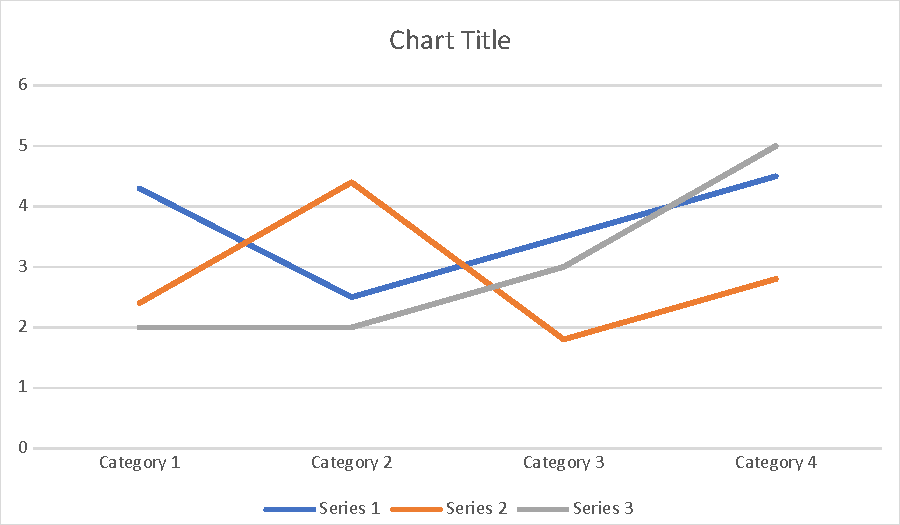
\includegraphics[width=15.24cm,height=8.89cm]{Gimbalscope20Dissertation20PreTex-img002.pdf} 

\captionof{figure}[This is an example figure caption]{\hypertarget{Toc98342041}{}This is an example figure caption}

\bigskip


\bigskip

\textcolor{black}{Lorem ipsum dolor sit amet, consectetuer adipiscing elit. Aenean commodo ligula eget dolor. Aenean
massa. Cum sociis natoque penatibus et magnis dis parturient montes, nascetur ridiculus mus. Donec quam felis,
ultricies nec, pellentesque eu, pretium quis, sem. Nulla consequat massa quis enim. Donec pede justo, fringilla vel,
aliquet nec, vulputate eget, arcu. In enim justo, rhoncus ut, imperdiet a, venenatis vitae, justo. Nullam dictum felis
eu pede mollis pretium. Integer tincidunt. Cras dapibus. Vivamus elementum semper nisi. Aenean vulputate eleifend
tellus. Aenean leo ligula, porttitor eu, consequat vitae, eleifend ac, enim. Aliquam lorem ante, dapibus in, viverra
quis, feugiat a, tellus. Phasellus viverra nulla ut metus varius laoreet. Quisque rutrum. Aenean imperdiet. Etiam
ultricies nisi vel augue. Curabitur ullamcorper ultricies nisi. Nam eget dui. Etiam rhoncus. Maecenas tempus, tellus
eget condimentum rhoncus, sem quam semper libero, sit amet adipiscing sem neque sed ipsum. Nam quam nunc, blandit vel,
luctus pulvinar, hendrerit id, lorem. Maecenas nec odio et ante tincidunt tempus. Donec vitae sapien ut libero
venenatis faucibus. Nullam quis ante. Etiam sit amet orci eget eros faucibus tincidunt. Duis leo. Sed fringilla mauris
sit amet nibh. Donec sodales sagittis magna. Sed consequat, leo eget bibendum sodales, augue velit cursus nunc,}


\bigskip

for ( i = 0; i {\textless} n; i++ ) \{ 

t[ i ] = 0; 

\} 

{\itshape\color[rgb]{0.26666668,0.32941177,0.41568628}
Listing \stepcounter{Listing}{\theListing}: This is an example listing}


\bigskip


\bigskip

\subsubsection{Example sub-section}
\hypertarget{Toc98342036}{}
\bigskip

\textcolor{black}{This is an example sub-section. }Lorem ipsum dolor sit amet, consectetuer adipiscing elit. Aenean
commodo ligula eget dolor. Aenean massa. Cum sociis natoque penatibus et magnis dis parturient montes, nascetur
ridiculus mus. Donec quam felis, ultricies nec, pellentesque eu, pretium quis, sem. Nulla consequat massa quis enim.
Donec pede justo, fringilla vel, aliquet nec, vulputate eget, arcu. In enim justo, rhoncus ut, imperdiet a, venenatis
vitae, justo. Nullam dictum felis eu pede mollis pretium. Integer tincidunt. Cras dapibus. Vivamus elementum semper
nisi. Aenean vulputate eleifend tellus. Aenean leo ligula, porttitor eu, consequat vitae, eleifend ac, enim. Aliquam
lorem ante, dapibus in, viverra quis, feugiat a, tellus. Phasellus viverra nulla ut metus varius laoreet. Quisque
rutrum. Aenean imperdiet. Etiam ultricies nisi vel augue. Curabitur ullamcorper ultricies nisi. Nam eget dui. Etiam
rhoncus. Maecenas tempus, tellus eget condimentum rhoncus, sem quam semper libero, sit amet adipiscing sem neque sed
ipsum. Nam quam nunc, blandit vel, luctus pulvinar, hendrerit id, lorem. Maecenas nec odio et ante tincidunt tempus.
Donec vitae sapien ut libero venenatis faucibus. Nullam quis ante. Etiam sit amet orci eget eros faucibus tincidunt.
Duis leo. Sed fringilla mauris sit amet nibh. Donec sodales sagittis magna. Sed consequat, leo eget bibendum sodales,
augue velit cursus nunc, Lorem ipsum dolor sit amet, consectetuer adipiscing elit. Aenean commodo ligula eget dolor.
Aenean massa. Cum sociis natoque penatibus et magnis dis parturient montes, nascetur ridiculus mus. Donec quam felis,
ultricies nec, pellentesque eu, pretium quis, sem. Nulla consequat massa quis enim. Donec pede justo, fringilla vel,
aliquet nec, vulputate eget, arcu. In enim justo, rhoncus ut, imperdiet a, venenatis vitae, justo. Nullam dictum felis
eu pede mollis pretium. Integer tincidunt. Cras dapibus. Vivamus elementum semper nisi. Aenean vulputate eleifend
tellus. Aenean leo ligula, porttitor eu, consequat vitae, eleifend ac, enim. Aliquam lorem ante, dapibus in, viverra
quis, feugiat a, tellus. Phasellus viverra nulla ut metus varius laoreet. Quisque rutrum. Aenean imperdiet. Etiam
ultricies nisi vel augue. Curabitur ullamcorper ultricies nisi. Nam eget dui. Etiam rhoncus. Maecenas tempus, tellus
eget condimentum rhoncus, sem quam semper libero, sit amet adipiscing sem neque sed ipsum. Nam quam nunc, blandit vel,
luctus pulvinar, hendrerit id, lorem. Maecenas nec odio et ante tincidunt tempus. Donec vitae sapien ut libero
venenatis faucibus. Nullam quis ante. Etiam sit amet orci eget eros faucibus tincidunt. Duis leo. Sed fringilla mauris
sit amet nibh. Donec sodales sagittis magna. Sed consequat, leo eget bibendum sodales, augue velit cursus nunc,


\bigskip


\bigskip

\textbf{for} \textit{i = 0} \textbf{upto} \textit{n} \textbf{do} 

t\textsubscript{i }$\leftarrow $ 0 

\textbf{end }

{\itshape\color[rgb]{0.26666668,0.32941177,0.41568628}
\textcolor{black}{Algorithm \stepcounter{Algorithm}{\theAlgorithm}\ Example algorithm}}


\bigskip


\bigskip

\paragraph{Example sub-sub-section}

\bigskip

\textcolor{black}{This is an example sub-sub-section. }Lorem ipsum dolor sit amet, consectetuer adipiscing elit. Aenean
commodo ligula eget dolor. Aenean massa. Cum sociis natoque penatibus et magnis dis parturient montes, nascetur
ridiculus mus. Donec quam felis, ultricies nec, pellentesque eu, pretium quis, sem. Nulla consequat massa quis enim.
Donec pede justo, fringilla vel, aliquet nec, vulputate eget, arcu. In enim justo, rhoncus ut, imperdiet a, venenatis
vitae, justo. Nullam dictum felis eu pede mollis pretium. Integer tincidunt. Cras dapibus. Vivamus elementum semper
nisi. Aenean vulputate eleifend tellus. Aenean leo ligula, porttitor eu, consequat vitae, eleifend ac, enim. Aliquam
lorem ante, dapibus in, viverra quis, feugiat a, tellus. Phasellus viverra nulla ut metus varius laoreet. Quisque
rutrum. Aenean imperdiet. Etiam ultricies nisi vel augue. Curabitur ullamcorper ultricies nisi. Nam eget dui. Etiam
rhoncus. Maecenas tempus, tellus eget condimentum rhoncus, sem quam semper libero, sit amet adipiscing sem neque sed
ipsum. Nam quam nunc, blandit vel, luctus pulvinar, hendrerit id, lorem. Maecenas nec odio et ante tincidunt tempus.
Donec vitae sapien ut libero venenatis faucibus. Nullam quis ante. Etiam sit amet orci eget eros faucibus tincidunt.
Duis leo. Sed fringilla mauris sit amet nibh. Donec sodales sagittis magna. Sed consequat, leo eget bibendum sodales,
augue velit cursus nunc,


\bigskip

\captionof{figure}[Example table caption]{\hypertarget{Toc98342047}{}\textcolor{black}{Example table caption}}
\begin{flushleft}
\tablefirsthead{}
\tablehead{}
\tabletail{}
\tablelasttail{}
\begin{supertabular}{m{5.1270003cm}|m{5.1270003cm}|m{5.1270003cm}}
\multicolumn{1}{m{5.1270003cm}}{~
} &
\multicolumn{1}{m{5.1270003cm}}{~
} &
~
\\\hline
{\selectlanguage{english}\bfseries \textcolor{black}{Foo}} &
{\selectlanguage{english} \textcolor{black}{Bar}} &
{\selectlanguage{english} \textcolor{black}{Baz}}\\\hline
~
 &
~
 &
~
\\\hline
~
 &
~
 &
~
\\\hline
~
 &
~
 &
~
\\\hline
~
 &
~
 &
~
\\\hline
\end{supertabular}
\end{flushleft}

\bigskip

\clearpage\section{Chapter 4: Critical Evaluation}
\hypertarget{Toc98342037}{}
\bigskip

\textbf{\textcolor{black}{A topic-specific chapter}}


\bigskip

\textcolor{black}{This chapter is intended to evaluate what you did. \ The content is highly topic-specific, but for
many projects will have flavours of the following:}


\bigskip

\liststyleWWNumxviii
\begin{enumerate}
\item \textcolor{black}{functional testing, including analysis and explanation of failure cases,}
\item \textcolor{black}{behavioural testing, often including analysis of any results that draw some form of conclusion
wrt. the aims and objectives, and}
\item \textcolor{black}{evaluation of options and decisions within the project, and/or a comparison with alternatives.}
\end{enumerate}

\bigskip

\textcolor{black}{This chapter often acts to differentiate project quality: even if the work completed is of a high
technical quality, critical yet objective evaluation and comparison of the outcomes is crucial. In essence, the reader
wants to learn something, so the worst examples amount to simple statements of fact (e.g., ``graph X shows the result
is Y''); the best examples are analytical and exploratory (e.g., ``graph X shows the result is Y, which means Z; this
contradicts, which may be because I use a different assumption''). \ As such, both positive
}\textit{\textcolor{black}{and}}\textcolor{black}{ negative outcomes are valid
}\textit{\textcolor{black}{if}}\textcolor{black}{ presented in a suitable manner.}


\bigskip


\bigskip

\clearpage\section{Chapter 5: Conclusion}
\hypertarget{Toc98342038}{}
\bigskip

\textbf{\textcolor{black}{A chapter }}


\bigskip

\textcolor{black}{The concluding chapter of a dissertation is often underutilised because it is too often left too close
to the deadline: it is important to allocate enough attention to it. Ideally, the chapter will consist of three parts:}


\bigskip

\liststyleWWNumxx
\begin{enumerate}
\item \textcolor{black}{(Re)summarise the main contributions and achievements, in essence summing up the content.}
\item \textcolor{black}{Clearly state the current project status (e.g., ``X is working, Y is not'') and evaluate what
has been achieved with respect to the initial aims and objectives (e.g., ``I completed aim X outlined previously, the
evidence for this is within Chapter Y''). \ There is no problem including aims which were not completed, but it is
important to evaluate and/or justify why this is the case.}
\item \textcolor{black}{Outline any open problems or future plans. Rather than treat this only as an exercise in what
you }\textit{\textcolor{black}{could}}\textcolor{black}{ have done given more time, try to focus on any unexplored
options or interesting outcomes (e.g., ``my experiment for X gave counter-intuitive results, this could be because Y
and would form an interesting area for further study'' or ``users found feature Z of my software difficult to use,
which is obvious in hindsight but not during at design stage; to resolve this, I could clearly apply the technique of
Smith [7]'').}
\end{enumerate}

\bigskip


\bigskip

\clearpage
\bigskip

\section{Bibliography}
\hypertarget{Toc98342039}{}\bibliographystyle{plain}
\bibliography{Gimbalscope20Dissertation20PreTex}

\bigskip

\clearpage
\bigskip


\bigskip

\section{Appendix A: An Example Appendix}
\hypertarget{Toc98342040}{}
\bigskip


\bigskip

\textcolor{black}{Content which is not central to, but may enhance the dissertation can be included in one or more
appendices; examples include, but are not limited to}


\bigskip

\liststyleWWNumxix
\begin{itemize}
\item \textcolor{black}{lengthy mathematical proofs, numerical or graphical results which are summarised in the main
body,}
\item \textcolor{black}{sample or example calculations, and}
\item \textcolor{black}{results of user studies or questionnaires.}
\end{itemize}

\bigskip

\textcolor{black}{Note that in line with most research conferences, the marking panel is not obliged to read such
appendices.}


\bigskip


\bigskip


\bigskip
\end{document}
